\fancyhead[L]{\textsf{\textbf{BÀI 1.2}}\hspace{1em}\textsf{Mô hình toán học: Danh mục các hàm cơ bản}}
\fancyhead[R]{\textbf{\textsf{23}}}
\noindent
\begin{minipage}[t][0.88\textheight][t]{0.26\textwidth}
    \vspace*{3.2cm}
    \centering
    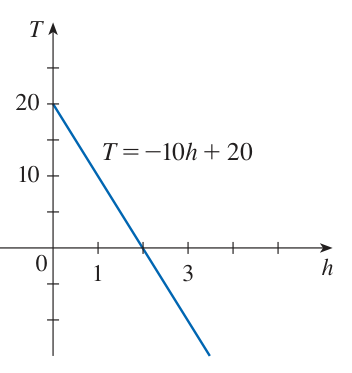
\includegraphics[width=0.9\linewidth]{images/p0058_fig1.png}
    \vspace{-0.2em}
    \begin{flushleft}
        \textbf{\textsf{HÌNH 3}}
    \end{flushleft}

    \vspace{1.8cm}

    {\footnotesize
    \centering
    \textbf{\textsf{Bảng 1}}
    \vspace{0.2em}

    \setlength{\tabcolsep}{2.5pt}
    \renewcommand{\arraystretch}{1.05}
    \begin{tabular}{|c|c|c|c|}
    \hline
    \rowcolor{stewartcyan!20}
    Năm & \makecell{Nồng độ\\$\text{CO}_2$\\ (ppm)} & Năm & \makecell{Nồng độ\\$\text{CO}_2$\\ (ppm)} \\
    \hline
    1980 & 338{,}7 & 2000 & 369{,}4 \\
    1984 & 344{,}4 & 2004 & 377{,}5 \\
    1988 & 351{,}5 & 2008 & 385{,}6 \\
    1992 & 356{,}3 & 2012 & 393{,}8 \\
    1996 & 362{,}4 & 2016 & 404{,}2 \\
    \hline
    \end{tabular}
    }

    \vfill

    \begin{flushright}
        \textbf{\textsf{HÌNH 4}}\\[0.2em]
        {\scriptsize Biểu đồ phân tán nồng độ $\text{CO}_2$ trung bình}
    \end{flushright}
    \vspace*{0.5cm}
\end{minipage}%
\hfill
\begin{minipage}[t][0.88\textheight][t]{0.71\textwidth}
    \vspace{0pt}
    \noindent\textbf{\textsf{\color{stewartcyan}VÍ DỤ 1}}
    \begin{enumerate}[(a)]
        \setlength{\itemsep}{1pt}
        \setlength{\parsep}{0pt}
        \setlength{\topsep}{2pt}
        \item Khi không khí khô bốc lên cao, nó giãn nở và lạnh đi. Nếu nhiệt độ mặt đất là $20^\circ\text{C}$ và nhiệt độ ở độ cao $1\text{ km}$ là $10^\circ\text{C}$, hãy biểu diễn nhiệt độ $T$ (theo $^\circ\text{C}$) như một hàm số của độ cao $h$ (tính bằng kilômét), giả sử rằng một mô hình tuyến tính là phù hợp.
        \item Vẽ đồ thị của hàm số trong câu (a). Hệ số góc biểu diễn cho điều gì?
        \item Nhiệt độ ở độ cao $2{,}5\text{ km}$ là bao nhiêu?
    \end{enumerate}

    \vspace{0.2em}
    \noindent\textbf{\textsf{\color{stewartcyan}LỜI GIẢI}}
    \begin{enumerate}[(a)]
        \setlength{\itemsep}{2pt}
        \setlength{\parsep}{0pt}
        \setlength{\topsep}{2pt}
        \item Vì chúng ta giả thiết rằng $T$ là một hàm tuyến tính của $h$, ta có thể viết
        \[
        T = mh + b
        \]
        Theo đề bài, $T = 20$ khi $h = 0$, do đó
        \[
        20 = m \cdot 0 + b = b
        \]
        Nói cách khác, tung độ gốc là $b = 20$.

        Ta cũng có $T = 10$ khi $h = 1$, do đó
        \[
        10 = m \cdot 1 + 20
        \]
        Vì vậy, hệ số góc của đường thẳng là $m = 10 - 20 = -10$ và hàm tuyến tính cần tìm là
        \[
        T = -10h + 20
        \]

        \item Đồ thị được vẽ trong Hình 3. Hệ số góc là $m = -10^\circ\text{C/km}$, đại diện cho tốc độ thay đổi của nhiệt độ theo độ cao.

        \item Ở độ cao $h = 2{,}5\text{ km}$, nhiệt độ là
        \[
        T = -10(2{,}5) + 20 = -5^\circ\text{C} \tag*{{\color{stewartcyan}$\blacksquare$}}
        \]
    \end{enumerate}

    \vspace{0.3em}
    Nếu không có định luật hay nguyên lý vật lý nào giúp ta xây dựng mô hình, ta sẽ lập một \textbf{mô hình thực nghiệm} (\textit{empirical model}), mô hình này hoàn toàn dựa trên dữ liệu thu thập được. Chúng ta tìm kiếm một đường cong ``khớp'' với dữ liệu theo nghĩa là nó phản ánh được xu hướng cơ bản của các điểm dữ liệu.

    \vspace{0.6em}
    \noindent\textbf{\textsf{\color{stewartcyan}VÍ DỤ 2}}\hspace{0.5em} Bảng 1 liệt kê nồng độ carbon dioxide trung bình trong khí quyển, được đo bằng phần triệu (ppm) tại Đài quan sát Mauna Loa từ năm 1980 đến năm 2016. Hãy sử dụng dữ liệu trong Bảng 1 để tìm một mô hình cho nồng độ carbon dioxide.

    \vspace{0.3em}
    \noindent\textbf{\textsf{\color{stewartcyan}LỜI GIẢI}}\hspace{0.5em} Chúng ta sử dụng dữ liệu trong Bảng 1 để vẽ biểu đồ phân tán trong Hình 4, trong đó $t$ biểu diễn thời gian (tính bằng năm) và $C$ biểu diễn nồng độ $\text{CO}_2$ (tính bằng phần triệu, ppm).

    \vspace{0.4em}
    \noindent
    \centering
    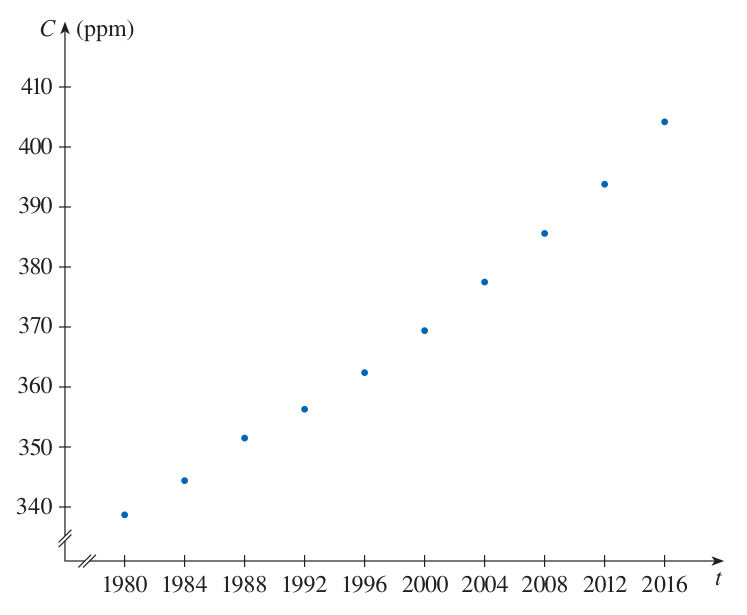
\includegraphics[width=0.92\linewidth]{images/p0058_fig2.png}
\end{minipage}